\begin{figure}[h]
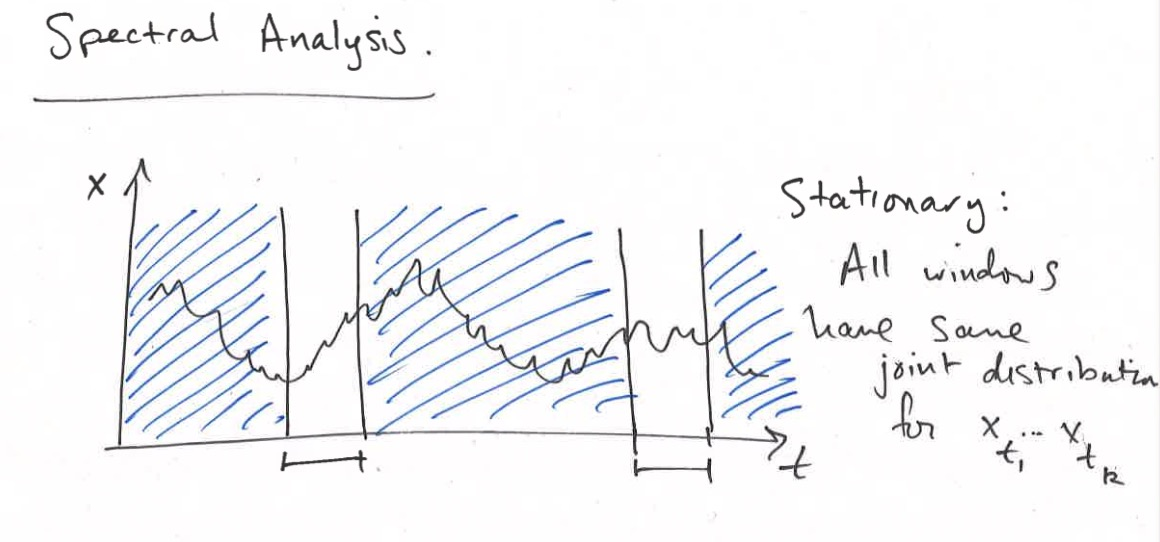
\includegraphics[scale=0.3]{images/Screenshot 2024-04-29 at 08.36.41.jpg}
\centering
\end{figure}


\underline{Question:} \quad Is the following time series stationary:\\
\begin{itemize}
    \item[] Let $R>0$ be a positive random variable.
    \item[] Let $\phi \in [0, 2\pi]$ be a uniform random variable
    \item[] Let $\varepsilon_t$ $t \in Z$ (so $t=...,-2-1,0,1,2,...$)
    \item[] \[X_t = R \cdot cos(t+ \phi) + \varepsilon_t\] 
    \item[] Note: this is stationary: why? 
    \item[] Compare to $W_t = cos(t)+ \varepsilon_t$ (i.e., $R=1, \phi = 0$ instead of random) $\Rightarrow$ Not-stationary 
\end{itemize}

\begin{figure}[h]
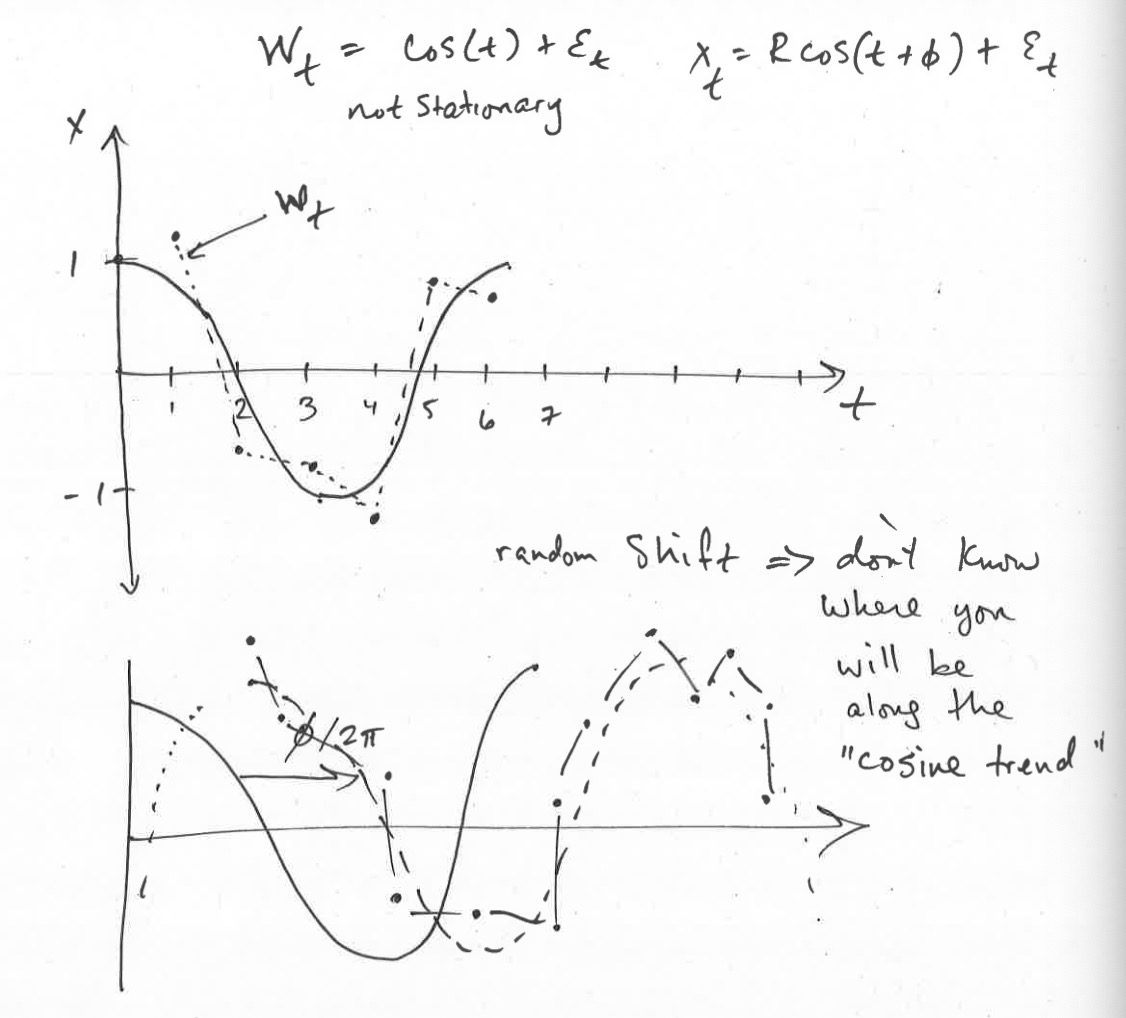
\includegraphics[scale=0.25]{images/Screenshot 2024-04-29 at 08.38.34.jpg}
\centering
\end{figure}

\begin{figure}[h]
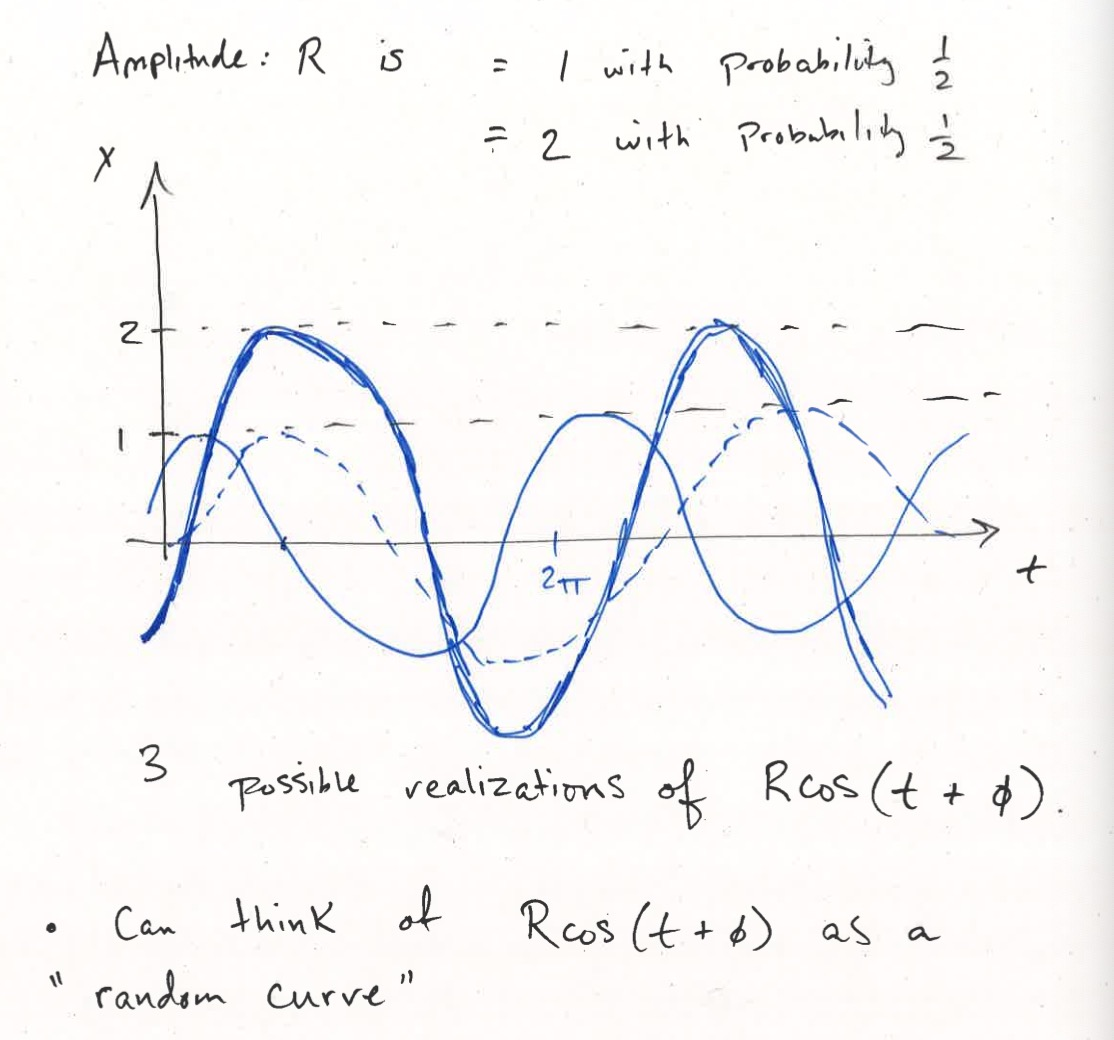
\includegraphics[scale=0.25]{images/Screenshot 2024-04-29 at 08.38.59.jpg}
\centering
\end{figure}



\underline{Question:} Can all stationary time series be decomposed into a sequence of random curves of the form $R(cos(wt + \phi))$ ? 

\[X_t = \sum_{j=1}^k R_j cos(w_j t +\phi_j)+Z_t \]
\quad with $w_j$ deterministic frequencies and $R_j, \phi_j$ random amplitudes and phases and $Z_t$ idiosyncratic or iid. 

\underline{Answer:} In a certain sense, yes: \\
\quad But have to let $k\rightarrow \infty$ and take a limit in the right way. \\

Implications: \quad Let $X_t$ be a stationary process with finite moments. Let $\gamma(k)$ be its autocovariance function. \[
\gamma(k) = cov(X_t, X_{t-k})
\]
Then there is an increasing function $F(\omega)$ such that \[
\gamma(k) = \int_0^\pi cos(\omega k)d F(\omega)
\]

If $F$ is smooth, can take $f(\omega) = F'(\omega)$ and then \[
\gamma(k)=\int_0^\pi cos(\omega k) f(\omega) d\omega
\]
$f(\omega)$ is called the \textbf{\underline{Spectral density}}.\\
$f$ is the Fourier transform of $\gamma$ 
\begin{align*}
\underbrace{f}_\text{spectral density}(\underbrace{\omega}_\text{frequency}) &= \frac{1}{\pi} \sum_{k=-\infty}^{\infty} \gamma(k)^{\overbrace{i}^\text{$i=\sqrt{-1}$}\omega k}\\
\Rightarrow f(\omega)&= \frac{1}{\pi}[\gamma(0)+2\sum_{k=1}^{\infty} \gamma(k) cos(\omega k) ]
\end{align*}
because $e^{-i\omega k}=cos(\omega k) + i sin(\omega k)$ and $\gamma(k) = \gamma(-k)$ so "sin" terms cancel. \\

Our representation theorem says: "Every stationary time series is approximately the sum of random cosine functions"

\begin{figure}[H]
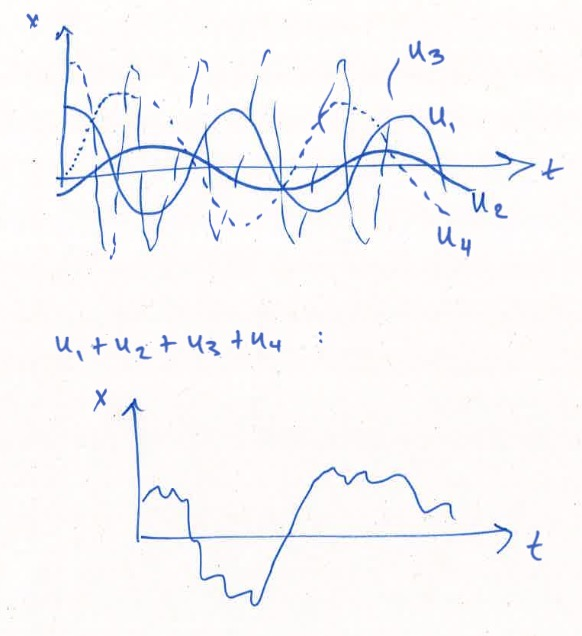
\includegraphics[scale=0.3]{images/Screenshot 2024-04-29 at 08.42.31.jpg}
\centering
\end{figure}


\underline{Ex.} Spectrum for white noise process:
\begin{align*}
    f(\omega)&=\frac{1}{\pi} \sum_{k=-\infty}^\infty \gamma(k) e^{-i\omega k}\\
    \gamma(0) & \neq 0 &&\text{but $\gamma_k = 0$ \quad $\forall k\neq0$} \\
    &+ \frac{1}{\pi} \sum_{k\neq 0} \underbrace{\gamma(k)}_{=0} e^{-i\omega k} \\
    &= \frac{1}{\pi} \gamma(0)\\
    &= \frac{1}{\pi}var(X_t)
\end{align*}

\begin{figure}[h]
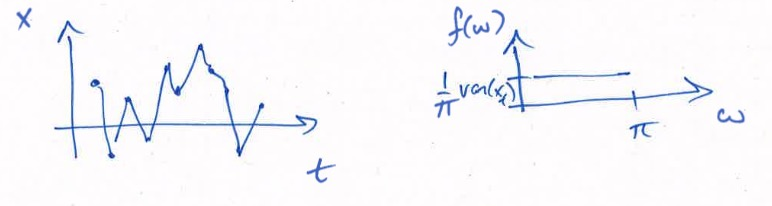
\includegraphics[scale=0.4]{images/Screenshot 2024-04-29 at 08.42.56.jpg}
\centering
\end{figure}


\subsection{Spectrum calculation for MA process}
\[X_t=\varepsilon_t + \theta \varepsilon_{t-1}\]
what is $\gamma(k)$?
\begin{align*}
    \gamma(1)&=cov(\varepsilon_t+\theta \varepsilon_{t-1}, \varepsilon_{t-1} \theta \varepsilon_{t-2} \\
    &= cov(X_t, _{t-1})\\
    &= cov(\varepsilon_{t}, \varepsilon_{t-1})+cov(\theta \varepsilon_{t-1}, \varepsilon_{t-1}) + cov(\varepsilon_{t}, \theta \varepsilon_{t-2}+cov(\theta \varepsilon_{t-1}, \theta \varepsilon_{t-2}\\
    &= \theta cov(\varepsilon_{t-1},\varepsilon_{t-1}) &&\text{(all other terms $=0$)}\\
    &= \theta var(\varepsilon_{t}\\
    \gamma(0)&= cov(\varepsilon_{t}, \theta \varepsilon_{t-1}, \varepsilon_{t} + \theta \varepsilon_{t-1}) \\
    &= (1+\theta^2)var(\varepsilon_{t}) \\
    \gamma(2)&=0 &&{\gamma(k)=0 \text{\quad} \forall |k|\geq 2 } \\
    \Rightarrow f(\omega) &= \frac{1}{\pi} [ 1 + \theta^2 + 2 \theta cos(\omega) ]var(\varepsilon_t)
\end{align*}

How to estimate $f(\omega)$ given data $X_1,...,X_T$?
\begin{align*}
    f(\omega) =\frac{1}{\pi} [ \gamma(o) + 2\sum_{k=1}^\infty \gamma(k) cos \omega k] 
\end{align*}

Two options for $\hat{f}$: 
\begin{enumerate}
    \item Truncate $\sum_{k=1}^\infty$ to $\sum_{k=1}^\mu$ for $M<<T$ to avoid degeneracy ($M=T$ doesn't work)
    \item Smoothed periodogram
\end{enumerate}

\underline{Periodogram}:
\begin{align*}
    I(\omega) &= \frac{1}{\pi T} \left | \sum_{t=1}^T X_t e^{i\omega t}\right |^2\\
    &= \frac{1}{\pi T} \left[ \left| \sum_{t=1}^T cos(\omega t)X_t + i sin(\omega t)X_t \right |^2 \right]
\end{align*}

\underline{Smoothed periodogram}:  \\

Smoothed version of $I(\omega)$\\

The value of the periodogram is 
\begin{align*}
    \underset{T\rightarrow\infty}{lim} E\left[I(\omega) \right] = f(\omega)
\end{align*}
Unfortunately, 

\[\underset{T \rightarrow \infty}{lim} var(I(\omega)) \neq 0 \]

But with Smoothing + the property that 
\[I(\omega_1) \overset{\ind}{\approx} I(\omega_2) \text{
\quad "$\overset{\ind}{\approx}$" means approximately independent. 
} \]


\[\Rightarrow \frac{1}{2a} \int_{\omega_0 - a}^{\omega_0 + a} I(\omega)d\omega \approx f(\omega_0) \text{\quad for a small $T$ with high probability.}\]
